\section{Problem Statement}
\label{sec:problem_definition}
Video surveillance in its current form is stationary, meaning cameras cannot move.
As a consequence of this, a large amount of hardware is required to properly surveil an area.
This is problematic when a large area has to be surveilled, as it requires a lot of hardware.
Drone technology offers a possible solution to this problem by making video surveillance dynamic through movable cameras.
This possible solution yields the following preliminary problem statement:\\

%http://guide-images.ifixit.net/igi/cI6EGVSLLjjDFATI.medium
\begin{figure}[htb]
    \centering
    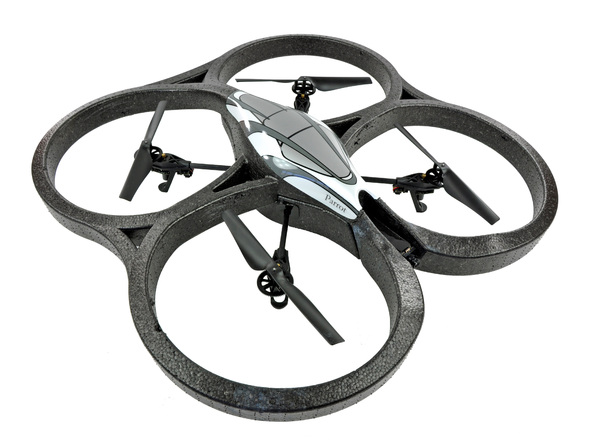
\includegraphics[width=\textwidth]{gfx/drone.jpg}
    \caption{A picture of the AR Drone 2.0 Parrot. Picture from: http://guide-images.ifixit.net/igi/cI6EGVSLLjjDFATI.medium}
    \label{fig:pic_of_drone}
\end{figure}

\textit{How can drone technology be applied in a software application to improve the efficiency of video surveillance?}\\

From the preliminary problem statement the following aspects must be considered:
\begin{itemize}
	\item How to control a drone through the web application
	\item How to provide video streaming of the drones camera through the web application
	\item How to make the web application scalable to support multiple drones and users
	\item How the make the system accessible from remote locations in a secure manner
\end{itemize}

For this project a AR Drone 2.0 Parrot, see Figure~\ref{fig:pic_of_drone}, has been acquired.

Section~\ref{sec:problem_definition} yields the following problem statement:

\textit{How can drone technology be applied in a web application to improve the efficiency and cost-efficiency of remote video surveillance of large out-door areas?}